\chapter{Inférence bayésienne et la théorie de la réponse aux items}
\label{chap:irt}
\minitoc
\thispagestyle{empty}
\newpage

\section{Introduction}
Lors du 25e anniversaire de la Psychometric Society en 1961, Harold Gulliksen a décrit « le problème de la théorie des tests » comme « la relation entre la capacité de l'individu et son score au test" (Gulliksen, 1961). Vingt-cinq ans plus tard, Charles Lewis a observé qu' « une grande partie des progrès récents de la théorie des tests a été réalisée en traitant l'étude de la relation entre les réponses à un ensemble d'items de test et un trait hypothétique (ou traits) d'un individu comme un problème d'inférence statistique" (Lewis, 1986), apportant ainsi des solutions à des problèmes autrefois insolubles tels que l'adaptation des tests aux candidats individuels (par exemple, Lord, 1980, chap. 10), le tri des relations dans les modèles de réussite dans les systèmes scolaires hiérarchiques (par exemple, Aitkin \& Longford, 1986) et l’estimation des paramètre des modèles IRT. Et les concepts et outils d'inférence statistique aider à expliquer les relations entre les preuves et l'inférence sur les connaissances, l'apprentissage et les réalisations des élèves que ce qui est traditionnellement associé à la théorie des tests standard et aux résultats standardisés \cite{mislevy1994evidence}. \\
L'inférence peut être défini comme un raisonnement à partir de ce que nous savons et de ce que nous observons jusqu'aux explications, conclusions ou prédictions parce que nous raisonnons toujours en présence d'incertitude et les informations avec lesquelles nous travaillons sont généralement incomplètes, peu concluantes, se prêtent à plus d’une explication. L’utilisation de l’inférence bayésienne permet donc d’estimer à partir d’observations les paramètres d’écrivant la distribution de probabilité en tenant compte des informations supplémentaire appelé aussi des informations apriori. Par exemple dans le cas où on cherche à estimer les paramètre \(\displaystyle \theta1 \) et \(\displaystyle \theta2 \) venant du problème où 30\% des machines à sous ont une probabilité \(\displaystyle \theta1 \)  de donner 1EUR, le reste a une probabilité \(\displaystyle \theta2 \).\\
L'évaluation pédagogique concerne l'inférence sur les connaissances, les compétences et les réalisations des élèves, c’est-à-dire qu’il existe un intérêt pour l'étude des variables latentes \cite{azevedo2011bayesian}, utilisé surtout dans La théorie de la réponse aux items (TRI). Parce que les données ne sont jamais aussi complètes et sans équivoque qu'elles garantissent la certitude, la théorie des tests a évolué en partie pour répondre aux questions de poids, de couverture et d'importation des données. Les concepts et techniques qui en résultent peuvent être considérés comme des applications de principes plus généraux d'inférence en présence d’incertitude. Comme le dit Glen Shafer (cité dans Pearl, 1988) « La probabilité n'est pas vraiment une question de nombres ; il s'agit de la structure du raisonnement. ». \\
Dans cette partie nous verrons l’inférence bayésienne appliquer à la théorie des réponses aux items et la plateforme Stan qui permet d’appliquer cette inférence à partir des données.\\

\section{Inférence bayésienne}
\subsection{Définition}
L'inférence bayésienne est une méthode d'apprentissage des valeurs des paramètres dans les modèles statistiques à partir de données. L'inférence bayésienne est une approche entièrement probabiliste, dont les résultats sont des distributions de probabilité. Une autre caractéristique distinctive de l'inférence bayésienne est l'utilisation d'informations a priori dans les analyses. L'inférence bayésienne ne concerne pas un modèle statistique particulier, en fait, une multitude de modèles statistiques et de machine learning (que ce soit : la régression linéaire, la régression logistique, les réseaux de neurones artificiels, ...) peuvent être « entrainé » de manière bayésienne ou non bayésienne. L'inférence bayésienne peut être résumée comme étant une méthode d'apprentissage à partir de données.

\subsection{probabilité conditionnelle et théorème de bayes}
Les probabilités conditionnelles jouent un rôle central dans le processus d'inférence sur le monde incertain. La probabilité conditionnelle est définie comme la probabilité qu'un événement ou un résultat se produise, sur la base de l'occurrence d'un événement ou d'un résultat précédent. La probabilité conditionnelle fait référence aux chances qu'un résultat se produise étant donné qu'un autre événement s'est également produit. Il est souvent indiqué comme la probabilité de B étant donné A et s'écrit P(B|A), où la probabilité de B dépend de celle que A se produise. La formule de la probabilité conditionnelle est :

\begin{equation}
	Pr(B|A) = \frac{Pr(A|B)}{Pr(A)}
	\label{conditionnelle_probability}
\end{equation}

Le théorème de Bayes , du nom du mathématicien britannique du XVIIIe siècle Thomas Bayes, est une formule mathématique permettant de déterminer la probabilité conditionnelle. Le théorème fournit un moyen de réviser les prédictions ou théories existantes (probabilités de mise à jour) compte tenu de preuves nouvelles ou supplémentaires. Dans de nombreux problèmes d'analyse de données, le théorème de bayes fourni la possibilité de déduire la valeur des paramètres d'un modèle à partir de données. Le théorème de bayes est défini par la formule suivante :

\begin{equation}
	Pr(B|A) = \frac{Pr(A|B)*Pr(B)}{Pr(A)}
	\label{theoreme_bayes}
\end{equation}
Ou \(\displaystyle Pr(B|A) \) est la probabilité de l’évènement B sachant A. L’équation \ref{theoreme_bayes} peut être interpréter comme suit :

\begin{equation}
	Pr(hypothesis|data) = \frac{Pr(data|hypothesis)*Pr(hypothesis)}{Pr(data)}
	\label{theoreme_bayes2}
\end{equation}


\(\displaystyle Pr(hypothesis|data) \) est la probabilité d’une hypothèse qu’on cherche sachant les données. En appliquant le théorème de Bayes, \(\displaystyle Pr(hypothesis|data) \)  est le produit de la probabilité des données sachant l’hypothèse \(\displaystyle Pr(data|hypothesis) \) qui peut être aussi un modèle et la probabilité de l’hypothèse \(\displaystyle Pr(hypothesis) \) ensuite divisé par la probabilité des données \(\displaystyle Pr(data) \). Cette hypothèse est généralement quelque chose d’inobservé ou inconnu qu’on cherche à obtenir à partir des données. Par exemple pour les modèles de régression linéaire, c’est les paramètres du modèle qu’on cherche à estimer. Le théorème de bayes permet donc d’obtenir la probabilité de l’hypothèse sachant les données récolter.

\subsection{L’approche Bayésienne}
L’approche Bayésienne se base sur l’idée d’avoir certaines croyances préalables sur le système et puis mettre à jour ces croyances sur la base des données observées. C’est-à-dire avoir des connaissances a priori sur les paramètres inconnus. Ces connaissances prennent la forme d’une loi sur l’espace des paramètres qui s’appelle la loi a priori. L’approche bayésienne cherche donc à combiner d’une part l’information empirique obtenu sur les paramètres et l’interprétation des valeurs plus subjective (il y’a certaines idées sur les valeurs que les paramètres pourrait avoir). Cette procédure de mise à jour est basée sur le théorème de Bayes.

\subsection{Théorème de bayes dans la cadre de l’application de l’approche Bayésienne}
En remplaçant hypothèse (hypothesis) par \(\displaystyle \theta \) de l’équation \ref{theoreme_bayes2} comme étant le paramètre à estimer on obtient donc :

\begin{equation}
	Pr(\theta|data) = \frac{Pr(data|\theta)*Pr(\theta)}{Pr(data)}
	\label{theoreme_bayes3}
\end{equation}
Où,
\begin{itemize}
    \item \(\displaystyle Pr(\theta|data) \) (Posterior distribution) : est la distribution à posteriori du paramètre \(\displaystyle \theta \). C’est l’estimation de \(\displaystyle \theta \) a posteriori (après avoir vu les données).
    \item \(\displaystyle Pr(data|\theta) \) (Likelihood) : c’est la vraisemblance qui est capturer à partir des données sachant le model utiliser pour faire l’inférence.
    \item \(\displaystyle Pr(\theta) \) (prior distribution) : c’est la distribution a priori sur le paramètre \(\displaystyle \theta \). 
    \item \(\displaystyle Pr(data) \) : qui est la probabilité des données.
\end{itemize}


\begin{figure}[H]
	\begin{center}
		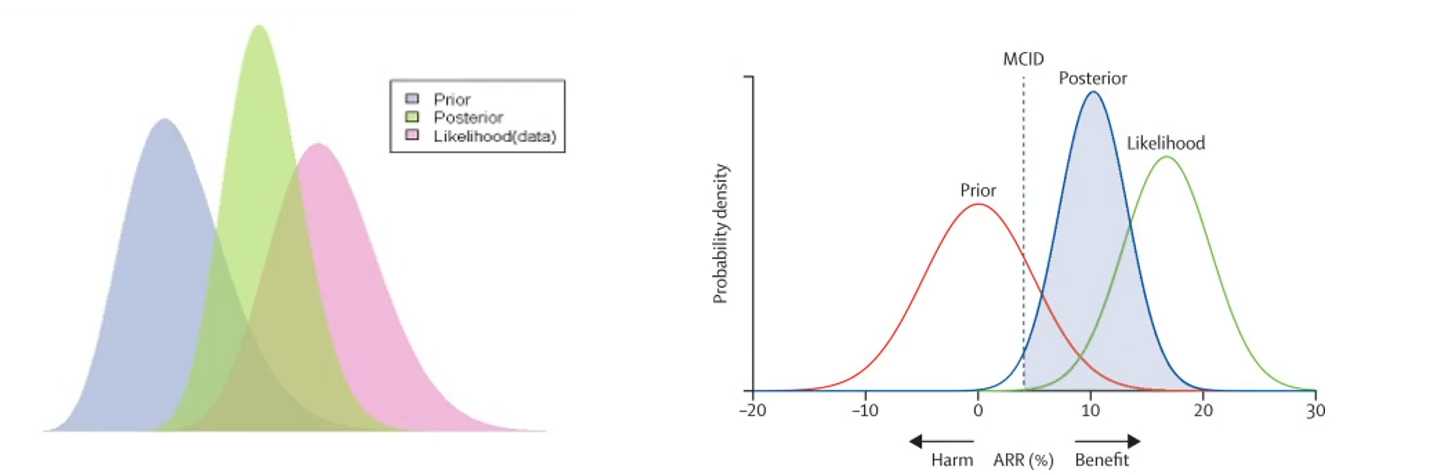
\includegraphics[width=\textwidth]{images/chapitre5/prior_likelihood_posterior.png}
	\end{center}
	\caption{La distribution à priori, à posteriori et celle de la fonction de vraisemblance.}
	\label{prior_likelihood_posterior}
\end{figure}

\subsubsection{Posterior distribution}
La probabilité postérieure est la probabilité qu'un événement se produise après que toutes les informations sur le système étudier aient été prises en compte. Elle est étroitement liée à la probabilité antérieure, qui est la probabilité qu'un événement se produise avant la pris en compte de nouvelles preuves. Elle est comme un ajustement sur la probabilité antérieure.

\begin{equation}
    \begin{split}
		Posterior \hspace{5pt} probability = prior \hspace{5pt} probability + new \hspace{5pt} evidence. \\
        Posterior \hspace{5pt} Distribution = Prior \hspace{5pt} Distribution + Likelihood \hspace{5pt} Function.
	\end{split}
	\label{posterior_probability_distribution}
\end{equation}

Par exemple, les données historiques suggèrent qu'environ 60\% des étudiants qui commencent l'université obtiendront leur diplôme dans les 6 ans. C'est la probabilité a priori. Cependant, ce chiffre est en réalité bien inférieur. Alors les preuves collecter peuvent suggérer que le chiffre réel est en fait plus proche de 50\% ; c'est la probabilité postérieure. \\
La distribution à posteriori est un moyen de résumer les connaissances ou les informations sur les quantités incertaines en analyse bayésienne. C'est une combinaison de la distribution a priori et de la fonction de vraisemblance, qui indique les informations contenues dans les données observées (les « nouvelles preuves »).

\subsubsection{Likelihood}
Habituellement lorsque l’on parle de distribution de probabilité, on suppose que nous connaissons les valeurs des paramètres. Aussi appelé fonction de vraisemblance (ou plus simplement vraisemblance), c’est une fonction des paramètres d'un modèle statistique calculée à partir de données observées \cite{fisher1922mathematical}. C’est-à-dire la probabilité d’observer les données sous un certain model. Par exemple, la probabilité des données sachant \(\displaystyle \theta \) en utilisant \ref{theoreme_bayes3}.
En inférence bayésienne, cette vraisemblance peut être interprète comme la densité de probabilité des données conditionnellement à une valeur des paramètres et comme une mesure de l'information apportée par les données sur la valeur des paramètres.

\subsubsection{Prior distribution}
La distribution à priori capture la connaissance ou l’information apriori. Elle permet de mettre en forme les connaissances ou les informations avant de faire l’expérimentation. Ces sont des distribution subjective sans tenir compte des données. \\
Ensuite Il y’a la probabilité des données, qui est défini par :

\begin{equation}
	Pr(data) = \int_{}^{}  \,L(data|\theta)Pr(\theta)d\theta .
	\label{probability_of_data}
\end{equation}

Le calcule d’une intégrale avec un seul paramètres (intégrale a une dimension) est possible mais lorsqu’il y’a plus d’un paramètre, cette dernière devient une intégrale multiple qui est difficile voire impossible à calculer. \\
L’approche Bayésienne d’aujourd’hui utilise des méthodes de simulation MCMC (chaine de Markov Monte Carlo) pour passer outre ce problème de calcule d’intégrale multiple. Nous verrons dans la section suivantes les chaines de Markov de Monte Carlo et leurs méthodes.

\subsubsection{Chaine de Markov Monte Carlo (MCMC)}
Malheureusement, dans la plupart des cas pratiques, il est impossible d’obtenir une solution analytique pour la distribution a posteriori. Le dénominateur sous la forme continue du théorème de Bayes consiste en une intégrale sur un espace potentiellement de grande dimension. L’un des moyens de résoudre ce problème est d’obtenir des échantillons de la distribution a posteriori. Parmi les approches les plus utilisées pour surmonter ces difficultés, on trouve les méthodes du Monte Carlo par chaînes de Markov et l’inférence variationnelle (dont nous n’évoquerons pas). Les méthodes de Monte Carlo par chaîne de Markov (MCMC) proposent des schémas pour dessiner,tirer (draw en anglais qui est présent dans les objets fit des résultats d’échantillonnages) une série d'échantillons corrélés qui convergent vers la distribution cible \cite{neal1993probabilistic}. \\

Les algorithmes MCMC consistent à simuler séquentiellement une seule chaîne de Markov dont la distribution limite est celle choisie (par example, le maximum de la fonction de vraisemblance fois une densité de probabilité a priori des paramètres). Plus précisément, une chaîne de Markov est une séquence de variables aléatoires telle que la valeur suivante ou état de la séquence dépend uniquement de l’état présent et non des états passés \cite{neal1993probabilistic}. Alors, une séquence de variables aléatoires est générée \(\displaystyle \widehat{q}_{0}, \widehat{q}_{1}, ... \)  telle que l’état suivant \(\displaystyle \widehat{q}_{t+1} \) avec \(\displaystyle t \geq 0  \) est distribué selon la probabilité de transition \(\displaystyle T(\widehat{q}_{t} \rightarrow \widehat{q}_{t+1}) \overset{def}{=} P(\widehat{q}_{t+1}|\widehat{q}_{t}) \) \cite{gbedo2017techniques} tout en visant la convergence de la chaine, c’est-à-dire que la chaîne est ergodique (stationnaire, irréductible et non périodique). \\

Une chaîne de Markov est définit par les valeurs initiales des distributions marginales des paramètres et la probabilité de transition entre deux états de l’espace des paramètres : \(\displaystyle T(\widehat{q} \rightarrow \widehat{q}^{\prime}) \), pour aller d’un état \(\displaystyle \widehat{q} \) à l’autre état \(\displaystyle \widehat{q}^{\prime} \). Les algorithmes MCMC sont généralement influencés lors de l’implémentation par le point de départ de la chaîne (ce qui conduit à une phase de « burn-in », comme l’illustre la figure \ref{mcmc_iterations}), par le choix de la probabilité de transition, le taux de convergence, l’acceptance de l’algorithme, etc. \\

\begin{figure}[H]
	\begin{center}
		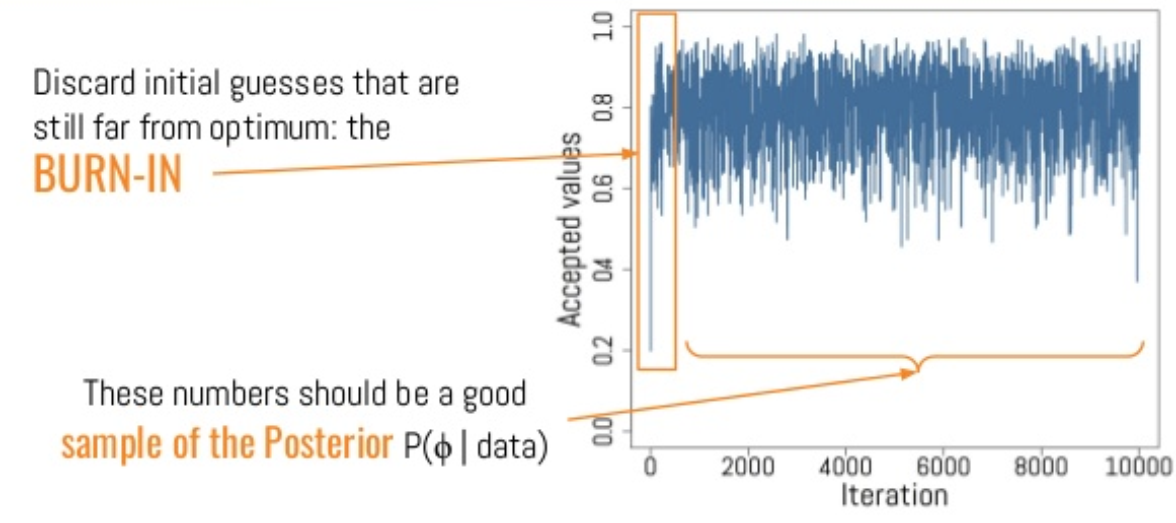
\includegraphics[width=\textwidth]{images/chapitre5/mcmc_iterations.png}
	\end{center}
	\caption{La phase « burn-in » d’une chaine de Markov et celle de la convergence de la chaine.}
	\label{mcmc_iterations}
\end{figure}

Les algorithmes de Monte Carlo à chaînes de Markov (MCMC) sont donc des outils informatiques standard pour analyser les modèles complexes bayésiens \cite{gelfand1990sampling} même si des fois des problème peuvent surgir dans leurs implémentations \cite{robert2020markov}. Parmi les méthodes MCMC, il y’a l’algorithme de Metropolis , l’algorithme de Metropolis–Hastings, échantillonnage de Gibbs, échantillonnage par tranches, Metropolis à tentatives multiples, Méthode de sur-relaxation l'hamiltonien Monte Carlo (HMC), No-U-Turn Sampler (NUTS), la méthode MCMC de Langevin et les méthodes basées sur le changement de dimension. Bien que notre travail ne soit pas centré sur les algorithmes MCMC, nous passerons en revue quelques définitions et théories qui justifient le fonctionnement des méthodes MCMC, et un bref résumé de quelque algorithmes MCMC. \\

\paragraph{Théorème de convergence des chaînes de Markov \cite{entezari2018bayesian} \cite{meyn2012markov} \cite{rosenthal2006first}}
Une chaîne de Markov à temps discret est définie par une séquence de variables aléatoires \(\displaystyle X_{0}, X_{2}, X_{3} ... \) qui peut prendre des valeurs possibles dans l'espace d'état \(\displaystyle X \) avec une distribution initiale définie pour \(\displaystyle X_{0}\) et des probabilités de transition définies comme :

\begin{equation}
	p(x,A) = P(X_{n+1} \in A | X_{n} = x), \hspace{1em} \forall A \subseteq X
\end{equation}
Où la propriété de Markov est :
\begin{equation}
	P(X_{n+1} \in A | X_{0},X_{1},...,X_{n}) = P(X_{n+1} \in A | X_{n})  \hspace{1em} \forall A \subseteq X
\end{equation}
Comme nous l’avons évoqué précédemment la probabilité que la chaîne passe à l'état suivant ne dépend que de l'état actuel et non des états précédents. \\
\textbf{\underline{Définition 1: }} Considérons une chaîne de Markov \(\displaystyle \left\{ X_{i} \right\} \) sur l'espace d'états \(\displaystyle X \) avec une probabilité de transition \(\displaystyle P(x,.) \). Soit \(\displaystyle \pi (.) \) une distribution de probabilité définie sur \(\displaystyle X \) . Alors \(\displaystyle \pi \) est une distribution stationnaire pour la chaîne de Markov  \(\displaystyle x,y \in X \) :

\begin{equation}
	\int_{x \in X}^{}  \,\pi(dx)P(x,dy) = \pi(dy)
\end{equation}

\noindent \textbf{\underline{Définition 2: }} Une chaîne de Markov est \(\displaystyle \phi \)-irréductible, s'il existe une mesure \(\displaystyle \sigma\)-finie non nulle sur \(\displaystyle X \) telle que :

\begin{equation}
	\begin{split}
	\forall A :  A \subseteq X \hspace{1em} avec \hspace{1em} \phi(A) > 0  \hspace{1em} \&  \hspace{1em} \forall x \in X \\
	\implies \exists \hspace{0.3em} n \in \mathbb{N} : P_{n}(x,A) > 0
	\end{split}
\end{equation}

\noindent \textbf{\underline{Définition 3: }} Une chaîne de Markov est apériodique, s'il n'y a pas de sous-ensembles disjoints non vides \(\displaystyle X_{1},...,X_{d} \subseteq X\) pour \(\displaystyle d \geq 2\) tel que \(\displaystyle P(x,X_{i+1}) = 1\) pour tout \(\displaystyle x \in X_{i} (1\leq i \leq d-1 ) \) et \(\displaystyle P(x,X_{1}) = 1 \) pour tout \(\displaystyle x \in X_{d}\). \\

\noindent \textbf{\underline{Théorème 1: }} Considérons une chaîne de Markov apériodique et \(\displaystyle \phi \)-irréductible définie sur un espace d'états \(\displaystyle X \) de distribution stationnaire \(\displaystyle \pi \). Pour \(\displaystyle \pi.a.e. \) \(\displaystyle x \in X \) :
\begin{equation}
	\lim_{x \to \infty} \left\lVert P^{n}(x,.) - \pi(.) \right\rVert = 0
\end{equation} 

\noindent Soit \(\displaystyle \lim_{x \to \infty} P^{n}(x,A) = \pi(A) \hspace{1em} \forall A \subseteq  X \) . \\
Dans la section suivante, nous décrirons quelques algorithmes MCMC les plus courants qui respectent l’aspect stationnaire, irréductible et non périodique des chaines de Markov.
\paragraph{Algorithme de Metropolis-Hastings}
L’algorithme de Metropolis-Hastings, proposé par METROPOLIS \cite{metropolis1953equation} et généralisé par HASTINGS \cite{hastings1970monte} est principalement utilisé comme moyen de simuler des observations à partir de distributions cibles. L'algorithme produit une chaîne de Markov dont la distribution limite des membres est la densité cible \(\displaystyle \pi(x) \) et qui s’itère en « sautant » de l’état actuel x de l’espace des paramètres à l’état suivant y avec une probabilité d’acceptation suivante :

\begin{equation}
	\alpha(x,y) = \min\Biggl( 1, \frac{\pi(y)q(y,x)}{\pi(x)q(x,y)} \Biggr)
\end{equation}

Où \(\displaystyle q(x,y) \) est la probabilité conditionnelle de proposer l'état \(\displaystyle y \) étant donné l'état \(\displaystyle x \). L'algorithme de Metropolis-Hastings est décrit dans l’algorithme \ref{m-c_algo}.

\begin{algorithm}
	\caption{Algorithme de Metropolis-Hastings \cite{entezari2018bayesian}}
	\label{m-c_algo}
	\begin{algorithmic}[1]
		\State Initial: value $X_{0}$, burn-in iterations $B$, number of samples $M$
		\State Output: $S_{1},...,S_{M}$ samples
		\For{$n$ in \{ $1,...,(B+M)$ \}}
			\State Draw $Y_{n}\sim Q(X_{n-1,.}) $, where $Q$ is the proposal distribution with probability density function q.
			\State Calculate $A_{n}$ = $\frac{\pi(Y_{n})q(Y_{n},Y_{n-1})}{\pi(X_{n-1})q(X_{n-1},Y_{n})}$
			\State Draw $U_{n} \sim $ Uniform[0,1]
			\If{$U_{n} < A_{n}$}
				\State $X_{n} = Y_{n}$ (« accept »)
			\Else
				\State $X_{n} = X_{n-1}$ (« reject »)
			\EndIf
		\EndFor
		\State \Return $S_{1} = X_{B+1},...,S_{M} = X_{B+M}$.
	\end{algorithmic}
\end{algorithm}

% \paragraph{Gibbs sampling}
\paragraph{Hamiltonian Monte Carlo}
L'hamiltonien Monte Carlo (HMC) est une méthode de Monte Carlo à chaîne de Markov (MCMC) capable de traiter des distributions cibles de grande dimension et qui utilise les dérivées de la fonction de densité échantillonnée pour générer des transitions efficaces couvrant la partie postérieure \cite{neal2011mcmc} \cite{betancourt2015hamiltonian}.Il utilise une simulation de dynamique hamiltonienne approximative basée sur une intégration numérique qui est ensuite corrigée en effectuant une étape d'acceptation Metropolis. Bien qu'il s'agisse d'un cas particulier d'échantillonneurs en temps continu, il peut être mis en œuvre en temps discret et est en fait à l'origine du succès du package Stan qui est utilisé dans la section implémentation \ref{irt_model_for_bayesian_inference}. L'hamiltonien Monte Carlo améliore l'efficacité en utilise le gradient du log postérieur pour diriger la chaîne de Markov vers les régions de densité postérieure plus élevée, où la plupart des échantillons sont prélevés, par conséquent, une chaîne HMC bien réglée acceptera les propositions à un taux beaucoup plus élevé que l'algorithme MH traditionnel \cite{gelman1997weak}. \\
Le processus repose sur une variable auxiliaire \(\displaystyle v \in \mathbb{R}^{d} \) qui augmente la distribution cible tout en échantillonnant à partir de \(\displaystyle \pi \) (une mesure cible de probabilité \(\displaystyle \pi \) sur \(\displaystyle \varTheta \subset \mathbb{R}_{d}\) par rapport à la mesure de Lebesgue, notée \(\displaystyle \pi(\theta) \infty \exp\{-U(\theta)\} \), où \(\displaystyle U \) est une fonction continûment dérivable appelée fonction de potentiel \cite{wu2018faster}. 
L’hamiltonien est défini par :
\begin{equation}
	H(\theta,v) = U(\theta) + \frac{1}{2}v^{T}M^{-1}v.
\end{equation}
\noindent Et HMC se base sur la dynamique hamiltonienne pour générer des propositions pour \(\displaystyle \theta \):
\begin{equation}
	\frac{d\theta}{dt} = \frac{\partial H}{\partial v} = M^{-1}v \hspace{0.5em} \text{et} \hspace{0.5em} \frac{dv}{dt} = - \frac{\partial H}{\partial \theta} = - \nabla U(\theta)
\end{equation}

\noindent L’algorithme HMC est :

\begin{algorithm}
	\caption{Algorithme de Monte Carlo hamiltonien \cite{wu2018faster}}
	\label{hmc_algo}
	\begin{algorithmic}[1]
		\State Initial: Starting point $\theta_{0}$ , step size $\epsilon $, number of leapfrog steps $L$, covariance matrix $M$, number of iterations $N$.
		\State Output: sample $\{ \theta_{0},...,\theta_{N}\}$ drawn from $\pi(\theta)$
		\For{$n \leftarrow 1$ to $N$}
			\State draw $v$ from $\mathcal{N}(\cdot|0,M)$ 
			\State compute $\theta^{\star},v^{\star} = Leapfrog(\theta_{n-1,v,\epsilon,L})$ compute
			\begin{equation}
				\rho = 1 \wedge \exp \{ H(\theta_{n-1},v) - H(\theta^{\star},-v^{\star})\}
			\end{equation}
			\State set
			\begin{equation}
				(\theta_{n},v_{n}) = \Biggl\{
				\begin{array}{ll}
					(\theta^{\star},-v^{\star}), \text{with probability} \rho \\
					(\theta_{n-1},v), \text{otherwise.}
				\end{array}
			\end{equation}
		\EndFor
		\State \Return $(\theta_{0},...,\theta_{N})$
		\Function{Leapfrog}{$\theta,v,\epsilon,L$}
			\State compute $(\theta_{0},v_{0}) = (\theta,v,- \epsilon / 2 \nabla U(\theta))$
			\For{$l \leftarrow 1$ to $L$}
				\State compute $\theta_{l} = \theta_{l-1} + \epsilon M^{-1}v_{l-1}$
				\State compute $v{l} = v_{l-1} -\epsilon \nabla U(\theta_{l})$
			\EndFor
			\State \Return $(\theta_{l},v_{l},+ \epsilon / 2 \nabla U(\theta_{l})$
		\EndFunction
	\end{algorithmic}
\end{algorithm}

\paragraph{No-U-Turn Sampler}
L’Hamiltonien Monte Carlo est un algorithme puissant, mais qui souffre de la nécessité d'ajuster le nombre d'étapes \(\displaystyle \mathcal{L}  \) par exemple en utilisant des heuristiques basées sur des statistiques d'autocorrélation à partir d'essais préliminaires coûteux \cite{neal2011mcmc}. Ce besoin de fixer le paramètre \(\displaystyle \mathcal{L}  \) est éliminé par l’algorithme No-U-Turn Sampler (NUTS). \\

Un échantillonneur MCMC qui utilise l’algorithme NUTS conserve la capacité de HMC à supprimer le comportement de marche aléatoire sans avoir besoin de définir le nombre \(\displaystyle \mathcal{L}  \) d'étapes de saut que l'algorithme prend pour générer une proposition. Le critère utilisé se base sur le produit scalaire entre \(\displaystyle \widetilde{r}  \) (la quantité de mouvement actuelle) et \(\displaystyle \widetilde{\theta} - \theta  \) (le vecteur de la position initiale à la position actuelle), qui est la dérivée par rapport au temps (dans le système hamiltonien) de la moitié de la distance au carré entre la position initiale \(\displaystyle \theta  \) et la position actuelle \(\displaystyle \widetilde{\theta}  \) \cite{hoffman2014no}:

\begin{equation}
	\frac{d}{dt} \frac{ (\widetilde{\theta} - \theta)^{T} (\widetilde{\theta} - \theta )}{2} = (\widetilde{\theta} - \theta)^{T} \frac{d}{dt} (\widetilde{\theta} - \theta) = (\widetilde{\theta} - \theta)^{T} \widetilde{r}.  
\end{equation}

\noindent Le pseudocode implémentant NUTS est fourni dans l'algorithme \ref{nuts_algo}. L'échantillonneur par défaut (NUTS) de Stan est plus efficace pour explorer le postérieur \cite{hoffman2011no}  \cite{hoffman2014no} et adapte automatiquement le nombre de pas de saut, éliminant le besoin de spécifier les paramètres de réglage par l'utilisateur.

\begin{algorithm}[H]
	\caption{No-U-Turn Sampler \cite{hoffman2011no}}
	\label{nuts_algo}
	\begin{algorithmic}[1]
		\State Resample $r \sim \mathcal{N} (0,I)$. ($I$ denote the identity matrix.)
		\State Resample $u \sim$ Uniform$(0,\exp\{\mathcal{L}(\theta^{t}) - \frac{1}{2}r^{T}r\})$. 
		\State Initalize $\theta^{-} = \theta^{t},\theta^{+} = \theta^{t}, r^{-} = r,r^{+} = r,j=0,\theta^{t+1} = \theta^{t},n=1,s=1.$
		\While{$s=1$}
			\State Chose a direction $v_{j} \sim$ Uniform$(\{-1,1\})$.
			\If{$v_{j} = -1$}
				\State $\{ \theta^{-},r^{-},-,-,\theta^{\prime},n^{\prime},s^{\prime} \} \leftarrow $ Recurse$(\theta^{-},r^{-},u,v_{j},j,\epsilon)$.
			\Else
				\State $\{ -,-,\theta^{+},r^{+},\theta^{\prime},n^{\prime},s^{\prime} \} \leftarrow $ Recurse$(\theta^{+},r^{+},u,v_{j},j,\epsilon)$.
			\EndIf
			\If{$s^{\prime} = 1$}
				\State With probability $\min\{ 1,\frac{n^{\prime}}{n} \}$, set $\theta^{t+1} \leftarrow \theta^{\prime} $.
			\EndIf
			\State $n \leftarrow n + n^{\prime}$.
			\State $s \leftarrow s^{\prime} \mathbb{I} \left[ (\theta^{+} - \theta^{-})^{T} r^{-} \geq 0  \right] \mathbb{I} \left[ (\theta^{+} - \theta^{-})^{T} r^{+} \geq 0  \right]  $.
			\State $j \leftarrow j+1$.
		\EndWhile
		\Function{Recurse}{$\theta,r,u,v,j,\epsilon$}
			\If{$j=0$}
				\State Base case take one leapfrog step in the direction v.
				\State $r^{\prime} \leftarrow \frac{v \epsilon}{2} \nabla_{\theta} \mathcal{L} (\theta)$.
				\State $\theta^{\prime} \leftarrow v \epsilon r^{\prime}$.
				\State $r^{\prime} \leftarrow \frac{v \epsilon}{2} \nabla_{\theta} \mathcal{L} (\theta^{\prime})$.
				\State $n^{\prime} \leftarrow \mathbb{I} \left[ u \leq \exp \{ \mathcal{L} (\theta^{\prime}) - \frac{1}{2} r^{\prime T} r^{\prime}\} \right] $.
				\State $s^{\prime} \leftarrow \mathbb{I} \left[ \mathcal{L} (\theta^{\prime}) - \frac{1}{2} r^{\prime T} r^{\prime} > u - \Delta_{\max}  \right] $
				\State \Return $\{ \theta^{\prime},r^{\prime},\theta^{\prime},r^{\prime},\theta^{\prime},n^{\prime},s^{\prime} \}$.
			\Else
				\State Recursion implicitly build the left and right subtrees.
				\State $\{ \theta^{-},r^{-},\theta^{+},r^{+},\theta^{\prime},n^{\prime},s^{\prime} \} \leftarrow $ Recurse$(\theta,r,u,v,j-1,\epsilon)$.
				\If{$s^{\prime} = 1$}
					\If{$v = -1$}
						\State $\{ \theta^{-},r^{-},-,-,\theta^{\prime \prime},n^{\prime \prime},s^{\prime \prime} \} \leftarrow $ Recurse$(\theta^{-},r^{-},u,v,j-1,\epsilon)$.
					\Else
						\State $\{ -,-,\theta^{+},r^{+},\theta^{\prime \prime},n^{\prime \prime},s^{\prime \prime} \} \leftarrow $ Recurse$(\theta^{+},r^{+},u,v,j-1,\epsilon)$.
					\EndIf
					\State With probability $\frac{n^{\prime \prime}}{n^{\prime} + n^{\prime \prime}}$, set $\theta^{\prime} \leftarrow \theta^{\prime \prime}$.
					\State $s \leftarrow s^{\prime \prime} \mathbb{I} \left[ (\theta^{+} - \theta^{-})^{T} r^{-} \geq 0  \right] \mathbb{I} \left[ (\theta^{+} - \theta^{-})^{T} r^{+} \geq 0  \right]  $. 
				\EndIf
				\State \Return $\{ \theta^{-},r^{-},\theta^{+},r^{+},\theta^{\prime},n^{\prime} + n^{\prime \prime},s^{\prime} \}$.
			\EndIf
		\EndFunction
	\end{algorithmic}
\end{algorithm}

% Malheureusement, dans la plupart des cas pratiques, il est impossible d'obtenir une solution analytique pour la distribution a posteriori. Le dénominateur sous la forme continue du théorème de Bayes consiste en une intégrale sur un espace potentiellement de grande dimension. L'un des moyens de résoudre ce problème est d'obtenir des échantillons de la distribution a posteriori. Ces échantillons sont distribués selon la distribution a posteriori.  \\
% Habituellement, les méthodes dites de Markov Chain Monte Carlo (MCMC) sont utilisées pour obtenir des échantillons à partir d'une distribution. Ces méthodes partent des valeurs initiales des paramètres. Ensuite, de nouvelles valeurs sont proposées et acceptées selon certaines fonctions de proposition et d'acceptation. Ce processus de proposition et d'acceptation est répété plusieurs fois pour créer un grand nombre d'échantillons. Différentes méthodes diffèrent principalement dans leurs implémentations des fonctions de proposition et d'acceptation. \\
% Les méthodes MCMC peuvent nécessiter un certain post-traitement des échantillons obtenus - par exemple, il peut être nécessaire d'ignorer les premiers (souvent des centaines ou des milliers) échantillons, car « ils ont été collectés loin des valeurs des paramètres pertinents » par exemple la figure ci-dessous. De plus, les échantillons sont généralement corrélés et donc souvent, seul un nième échantillon (après le retrait des échantillons initiaux) est retenu. De plus, les méthodes peuvent échouer (pour donner des échantillons représentatifs de la distribution). Il existe des moyens de diagnostiquer cela, par exemple en créant plusieurs « chaînes d'échantillonnage » (et en comparant leurs résultats). \\
%Plusieurs méthodes sont utilisées pour construire ces chaines comme : Metropolis-Hastings, Gibbs sampler, Metropolis-within-Gibbs, HMC etc.

\subsection{Méthodes de vérifications et de comparaison de modèles}
Les méthodes de vérifications de modèles sont différentes des méthodes de comparaisons du fait qu’elles permettent d'examiner si un modèle capture les caractéristiques importantes d'un ensemble de données, tandis que les méthodes de comparaisons répondent à la question de savoir quel modèle parmi un groupe de modèles candidats est le meilleur. \\
La théorie des réponses aux items (TRI) dans le cadre bayésien comme tout autres méthodes permettent une analyse plus approfondie en utilisant des distributions postérieures du modèle. En général, certaines techniques populaires de vérification de modèle bayésien qui ont été appliquées à l'IRT comprennent l'analyse résiduelle bayésienne, les vérifications prédictives préalables et les vérifications prédictives postérieures, et les méthodes de comparaison de modèles bayésiens incluent le critère d'information sur la déviance DIC \cite{spiegelhalter2003bayesian}, le facteur de Bayes \cite{kass1995bayes} et la probabilité de validation croisée et le facteur de Bayes partiel \cite{o1995fractional}. \\
Pour faire de la sélection de modèle (en comparant plusieurs modèles) il faut vérifier s’il y’a un effet des valeurs des paramètres sur la variable cible (par exemple sur la réussite ou pas à un item). \\
Dans le cadre fréquentiste, l’idée est de pénalisé les modèles qui ont trop de paramètres. Pour le faire il y’a \(\displaystyle AIC \)  :

\begin{equation}
	AIC = -2 \log (L(\widehat{\theta_{1}},...,\widehat{\theta_{k}} )) + 2K.
	\label{aic_formula}
\end{equation}

Avec \(\displaystyle L \) la vraisemblance et \(\displaystyle k \) le nombre de paramètres \(\displaystyle \theta \), et \\
\(\displaystyle -2 \log (L(\widehat{\theta_{1}},...,\widehat{\theta_{k}} )) \) est la déviance qui mesure la qualité de l’ajustement du model de donnée. Plus il y’a de paramètres plus cette quantité est petite et mieux le model est ajuster aux données. \\
\(\displaystyle 2k \) : c’est la pénalité, plus il y’a des paramètres plus cette quantité augmente. Cette pénalité est un équilibre entre l’ajustement du model des données et la complexité du model qui est capturer par le nombre de paramètres. \\ \\

\noindent En bayésien, le critère d'information WAIC (Watanabe Akaike Information Criteria) et la validation croisée LOO (leave-one-out cross-validation) sont considéré comme des méthodes de sélection de modèles entièrement bayésiennes en raison de leur utilisation de l'ensemble a posteriori distribution autre que les estimations ponctuelles. \\

\noindent WAIC \cite{watanabe2010asymptotic} est une méthode de sélection de modèle entièrement bayésienne basé sur un critère d'information et est considéré comme une version améliorée de DIC, définit comme suit :
%\noindent En bayésien il y’a WAIC (Watanabe Akaike Information Criteria) définit par :

\begin{equation}
	WAIC = -2\sum_{i=1}^{n} \log E\left[ p(y_{i}|\theta) \right] + 2p_{WAIC}
	\label{waic_formula}
\end{equation}

Où \(\displaystyle E\left[ p(y_{i}|\theta) \right] \) est la moyenne a posteriori de la vraisemblance de la ième observation.
\(\displaystyle Pwaic \)  est le nombre effectif de paramètres calculés en utilisant la variance postérieure de la vraisemblance.
La valeur de waic est la somme entre la deviance + le nombre de paramètre pwaic. \\

\noindent Une autre méthode de comparaison de modèles entièrement bayésienne est la validation croisée LOO \cite{geisser1979predictive} définit : \\

\begin{equation}
	LOO = -2\sum_{i=1}^{n} \log \int \,p(y_{i}|\theta)p_{post(-i)}(\theta)d\theta.
	\label{loo_formula}
\end{equation}
 Où \(\displaystyle p_{post(-i)}(\theta) \) est la distribution postérieure basée sur les données moins le point de données \(\displaystyle i \).
\section{La théorie des réponses aux items}
La théorie des réponses aux items (TRI) aussi appelé théorie des traits latents, théorie du vrai score fort ou théorie moderne des tests mentaux est un paradigme pour la conception, l’analyse et la notation des test et des questionnaires \cite{fisher1922mathematical}. TRI intervient dans la mesure ou la théorie classique n’apporte pas toujours des réponses satisfaisantes. Par exemple un item jugé facile ou difficile peut ne plus l’être dans un échantillon différent qu’il appartenait.

Dans cette situation, la théorie des réponses aux items tente de produire des propriétés de l’item qui soit indépendante d’un groupe particulier d’individus. En d'autres termes, il s'agit de parvenir à l'élaboration d'instruments de mesure dont les caractéristiques ne soient pas excessivement influencées par tel ou tel autre groupe de référence : ce qui, d'une certaine manière, conduit à définir des échelles qualifiées parfois d'"absolues" \cite{xcv_wiki}. La première tentative de développement de ce type d’échelle remontre au début des années 1950 (échelle de Guttman). Initialement, ils reposaient sur un modèle totalement déterministe qui a ensuite été remplacé par un modèle plus réaliste de type probabiliste (modèle de Rasch). Ces modèles reposent sur l’hypothèse selon laquelle la réponse d’un individu a un item est déterminée ou peut être expliquer par deux facteurs qui sont :

\begin{itemize}
	\item D’une part, certains attributs du sujet (sa compétence par exemple), qui, n'étant pas directement accessibles à l'observation et à la mesure, sont généralement qualifiés de traits latents \cite{xcv_wiki} ;
	\item D’autre part, les propriétés de l'item lui-même, notamment, sa difficulté, son pouvoir de discrimination, sans oublier le rôle que la "chance" (réponses "au hasard") peut jouer dans certains cas \cite{xcv_wiki}.
\end{itemize}

Sur le plan technique et mathématique, la théorie des réponses aux items utilise des modèles à un, deux ou trois paramètre(s), qui établissent la relation fondamentale entre le trait latent de l'individu (son niveau de compétence par exemple) et la probabilité pour cet individu de réussir un item donné. Cette relation est formalisée par une fonction (appelée fonction caractéristique de l'item), et peut être représentée géométriquement par une courbe (la courbe caractéristique de l'item). La forme la plus simple de cette fonction est celle qui repose sur le modèle de Rasch \cite{xcv_wiki}.\\
L'objectif de la méthode est double, il s'agit, d'une part, d'estimer les propriétés métriques des items (calcul des paramètres dits de difficulté, de discrimination et, éventuellement, de pseudo-chance) et, d'autre part, d'estimer le niveau de l'individu par rapport au trait latent considéré. Par ailleurs, ces estimations sont supposées indépendantes des échantillons particuliers (d'individus d'une part et d'items de l'autre) à partir desquels l'étude est réalisée \cite{xcv_wiki}.
\subsection{IRT dans la recherche organisationnelle}
Les modèles de la théorie des réponses aux items (TRI) présentent plusieurs avantages pour la recherche organisationnelle. L’un des avantages méthodologiques de l’IRT est la détection des réponses aberrante parmi d’autre avantage comme la construction et l’évaluation des échelles et l’examen des biais de mesure. Le tableau \ref{irt_application} présente un résumé de ces applications ainsi que quelques avantages par rapport aux approches alternatives.
\begin{table}[H]
	\centering
	\addtolength{\leftskip} {-4cm}
	\addtolength{\rightskip}{-4.5cm}
	\begin{tabular}{|m{4cm}|m{6cm}|m{6cm}|m{0.5cm}|}
	\hline
	\textbf{Problèmes méthodologiques} & \textbf{Applications de l'IRT} & \textbf{Avantages de l'IRT par rapport aux méthodes alternatives} & \\ \hline
	Construction et évaluation de l'échelle & 
	\begin{itemize}[leftmargin=*]
	    \item Peut être utilisé pour raccourcir une échelle ou examiner la qualité des échelles existantes
	    \item Peut être utilisé pour développer d'autres types d'évaluations.
	\end{itemize}
	& 
	\begin{itemize}[leftmargin=*]
		\item Contrairement au CTT, les paramètres des éléments IRT sont invariants d'un échantillon à l'autre.
		\item IRT peut être utilisé pour créer des tests adaptatifs, mais pas CTT.
		\item Bien que les méthodes CTT soient cohérentes avec les modèles de dominance, l'IRT peut être utilisé pour créer des mesures ponctuelles idéales.
	\end{itemize} & \cite{borman2001examination} \cite{carter2011using} \cite{chernyshenko2007constructing} \cite{roznowski1989examination} \cite{tay2009fitting}\\ \hline

	Identifier l'élément (l'item) et tester le biais &
	\begin{itemize}[leftmargin=*]
	    \item Peut différencier les différences moyennes observées du biais
	    \item Peut détecter les DIF et DTF compensatoires
	    \item Peut examiner les différences au niveau des options
	\end{itemize}
	&
	\begin{itemize}[leftmargin=*]
	    \item La comparaison des différences moyennes avec le CTT confond le biais avec de vraies différences dans le trait latent.
	    \item Les modalités d'examen du DTF sont plus développées qu'en CFA.
	\end{itemize}
	& \cite{chan1999shelf} \cite{nye2010never} \cite{raju2002measurement} \cite{stark2004examining} \cite{tay2015overview} \\ \hline

	Détection des réponses aberrantes &
	\begin{itemize}[leftmargin=*]
	    \item Peut être utilisé pour détecter différents types de réponses aberrantes telles que IER, falsification et réponse faussement faible.
	\end{itemize}
	&
	\begin{itemize}[leftmargin=*]
	    \item Les méthodes IRT peuvent détecter plusieurs types de réponses aberrantes tandis que d'autres méthodes ne peuvent détecter que des réponses imprudentes.
	    \item Les méthodes IRT sont souvent plus efficaces pour détecter les réponses aberrantes que les méthodes traditionnelles de réponse à l'effort insuffisant (IER).
	\end{itemize}
	& \cite{stark2001effects} \cite{drasgow1996optimal} \cite{zickar1999modeling} \cite{zickar2004uncovering} \\ \hline
    \end{tabular}
	\caption{Résumé des applications de l'IRT \cite{nye2020advancing}.}
	\label{irt_application}
\end{table}


\subsection{Les Modèles TRI}
On distingue deux familles de modèle IRT : les modèles unidimensionnels qui nécessitent une seule dimension de trait et les modèles multidimensionnels qui sont supposées provenir de plusieurs traits. Cependant, en raison de la complexité considérablement accrue, la majorité des recherches et des applications IRT utilisent un modèle unidimensionnel.
\subsubsection{Les modèles à un, deux ou trois paramètres}
Les modèles IRT se distingue par le nombre de paramètre qu’il utilise. Le modèle à paramètre unique (1PL) suppose tous les éléments qui correspondent au modèle ont la même difficulté, de sorte que ces éléments sont décrits par un seul paramètre. C’est le cas du modèle de Rasch. Le modèle dit à deux paramètre (2PL) fait appel au paramètre de difficulté et de discrimination par exemple le modèle de Birnbaum. Par contre le modèle a trois paramètres (3PL) est celui qui cherche à estimer en plus le paramètre de difficulté et de discrimination, la pseudo chance. \\
Il en résulte des modèles à un paramètre ayant la propriété d'objectivité spécifique, ce qui signifie que le rang de la difficulté de l'item est le même pour tous les répondants indépendamment de la capacité, et que le rang de la capacité de la personne est le même pour les items indépendamment de la difficulté. Ainsi, les modèles à 1 paramètre (comme ceux de Rasch) sont indépendants de l'échantillon, une propriété qui n'est pas valable pour les modèles à deux et trois paramètres \cite{fisher1922mathematical}. \\
Le modèle général de Birnbaum, auquel le modèle de Rasch se rattache est plus complexe car il admet des courbes d’allures différentes pour chacun des items et suppose donc d’estimer plus d’un paramètre par item puisqu’il tient également compte du pouvoir discriminant de chacun d’eux. Le modèle proposé par Lazarsfeld est en quelque sorte une simplification du modèle général de Birnbaum puisqu’il postule des distributions linéaires de pentes variables \cite{yvonnick_2019}. \\
Il existe aussi d’autre modèles IRT qui sont résumé dans le tableau \ref{irt_modeles}.

\begin{table}[H]
	\centering
	\addtolength{\leftskip} {-4cm}
	\addtolength{\rightskip}{-4.5cm}
	\begin{tabular}{|m{4cm}|m{6cm}|m{6cm}|}
	\hline
	\textbf{Modèle IRT} & \textbf{Description} & \textbf{Application} \\ \hline
	% Modèle logistique à un paramètre (One-parameter logistic model \textbf{1PL}) & & \\ \hline
	% Modèle logistique à deux paramètres (Two-parameter logistic model \textbf{2PL}) & Suit un processus de réponse de dominance et suppose que tous les items varient en fonction de la discrimination \(\displaystyle (a_{i})\) et de la difficulté \(\displaystyle (b_{i})\). & Utilisé pour les éléments dichotomiques (par exemple, oui/non ou correcte/incorrecte) pour lesquels il est peu probable de deviner (par exemple, les questions ouvertes avec de nombreuses réponses possibles). \\ \hline
	% Modèle logistique à trois paramètres (Three-parameter logistic model \textbf{3PL}) & Suit un processus de réponse de dominance et suppose que tous les items varient en fonction de la discrimination \(\displaystyle (a_{i})\), de la difficulté \(\displaystyle (b_{i})\) et de la pseudo-chance \(\displaystyle (c_{i})\). & Utilisé pour les éléments dichotomiques pour lesquels des devinettes sont susceptibles de se produire (par exemple, éléments avec une bonne ou une mauvaise réponse ou des options de réponse oui/non).\\ \hline
	Modèle logistique multidimensionnel à deux paramètres (Multidimensional two-parameter logistic model \textbf{M2PL}) & Suit un processus de réponse de dominance et suppose que tous les items varient sur un vecteur de paramètres de discrimination \(\displaystyle (a_{i} = a_{1},...,a_{m} )\) et de difficulté \(\displaystyle (b_{i})\). & Utilisé pour les éléments dichotomiques où il est peu probable de deviner. Peut être utilisé lorsque les données sont multidimensionnelles.\\ \hline
	Modèle de réponse graduée (Graded response model \textbf{GRM}) & Suit un processus de réponse de dominance et suppose que tous les items varient en fonction de la discrimination \(\displaystyle (a_{i})\) et que chaque option de réponse varie en fonction de la difficulté \(\displaystyle (b_{ik})\). En d'autres termes, chaque élément aura un paramètre a et \(\displaystyle C - 1 \) paramètres \(\displaystyle b \), où \(\displaystyle C \) est le nombre total d'options de réponse. & Utilisé pour les éléments polytomiques avec trois options de réponse ou plus.\\ \hline
	Modèle de réponse graduée multidimensionnelle (Multidimensional graded response model \textbf{MGRM}) &Suit un processus de réponse de dominance et suppose que tous les items varient sur un vecteur de paramètres de discrimination \(\displaystyle (a_{i} = a_{1},...,a_{m} )\) et chaque option de réponse varie en fonction de la difficulté \(\displaystyle (b_{ik})\). Chaque élément aura un vecteur d'un paramètre pour chaque facteur latent et des paramètres \(\displaystyle C - 1 \) \(\displaystyle b \), où \(\displaystyle C \) est le nombre total d'options de réponse. & Utilisé pour les éléments polytomiques avec trois options de réponse ou plus. Peut être utilisé lorsque les données sont multidimensionnelles.\\ \hline
	Modèle de dépliage gradué généralisé (Generalized graded unfolding model \textbf{GGUM}) & Suit un processus de réponse ponctuelle idéal et suppose que tous les éléments varient en fonction de la discrimination \(\displaystyle (a_{i})\), de l'emplacement de l'élément \(\displaystyle (\delta_{i})\) et des seuils \(\displaystyle (\tau_{i1})\). & Peut être utilisé pour les éléments ponctuels idéaux dichotomiques ou polytomiques. \\ \hline
	\end{tabular}
	\caption{Résumé des quelques modèles IRT \cite{nye2020advancing}.}
	\label{irt_modeles}
\end{table}

\begin{figure}[H]
	\begin{center}
		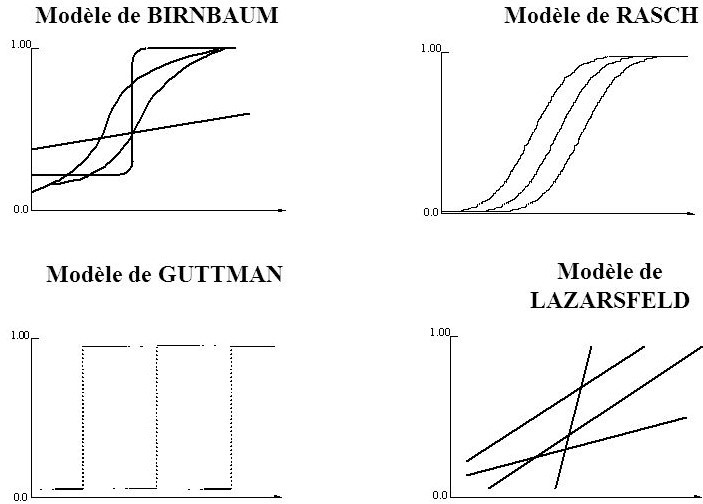
\includegraphics[width=\textwidth]{images/chapitre5/irt_models.jpg}
	\end{center}
	\caption{}
	\label{irt_models}
\end{figure}
\paragraph{Le modèle Rasch}
La structure cumulative ou d’emboitement des items obtenue par le scalogramme de Guttman rend les analyses exploratoires traditionnelles mal appropriées (AFC par exemple) . Dans cette situation Rasch a proposé en 1960 une représentation numérique des niveaux de compétences de sujets et de difficulté d’items. Le modèle de Rasch qui est le modèle a un paramètre (1PL), est considéré comme l’approche la plus simple pour modéliser la relation entre le trait latent et la probabilité de réussir correctement un item. Dans le modèle de Rasch chaque sujet est caractérisé par un niveau \(\displaystyle \theta i \) d’aptitude \(\displaystyle (i=1,...,N) \) sur un continuum numérique latent.
Le modèle de Rasch cherche a donné du sens non pas seulement au classement des sujets par compétences, non pas seulement au classement des items par difficultés mais le modèle cherche à donner du sens dans le fait que les coordonnées d’un sujet peuvent être directement et numériquement comparer à la difficulté d’un item pour qu’on puisse dire par exemple que ce sujet à la compétence nécessaire pour pouvoir résoudre l’item de tel difficulté. Donc ça devient possible de les comparer directement à partir du moment où on les projette sur une seule et même dimension (cet \(\displaystyle \theta i \) de sujet et \(\displaystyle \beta i \) d’item). La probabilité de réussir l’item est une fonction croissante de la différence \(\displaystyle \theta i - \beta j\) \cite{yvonnick_2019}.
Rasch propose la fonction logistique suivant \cite{mislevy1994evidence}:

\begin{equation}
    \begin{split}
		P(x_{1},...,x_{n} | \theta, \beta_{1},...,\beta_{n}) = \prod_{j=1}^{n} P(x_{j}| \theta, \beta_{j}), \hspace{10pt} avec, \\
		P(x_{j}| \theta, \beta_{j}) = \frac{\exp \left[x_{j}(\theta - \beta_{j})\right]  }{1+ \exp (\theta - \beta_{j})}
	\end{split}
	\label{posterior_probability_distribution}
\end{equation}

\begin{figure}[H]
	\begin{center}
		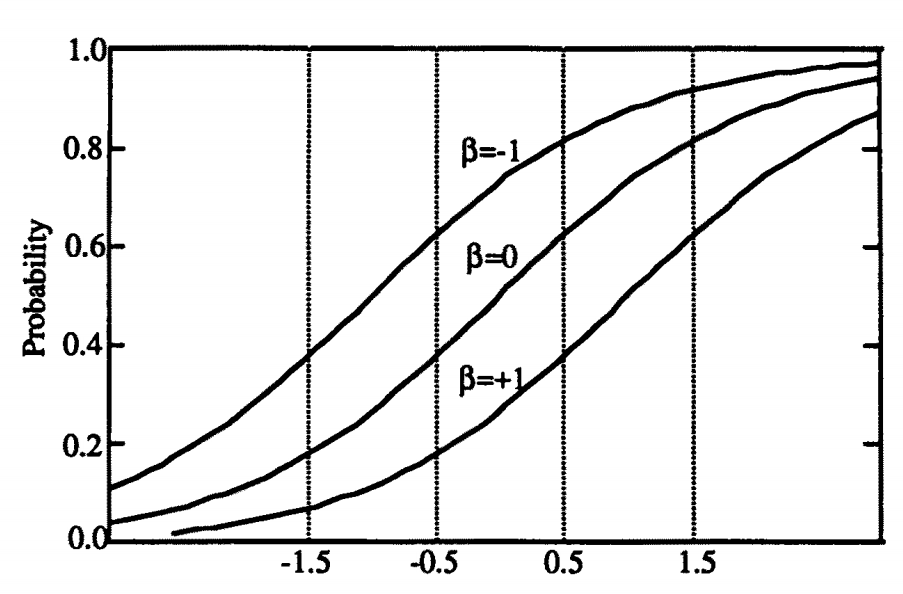
\includegraphics[width=\textwidth]{images/chapitre5/parameters_probability.png}
	\end{center}
	\caption{}
	\label{parameters_probability}
\end{figure}
Où \(\displaystyle x_{j} \)  est la réponse à l'élément \(\displaystyle j \) (1 pour correcte, 0 pour incorrecte). La figure \ref{parameters_probability} montre les probabilités de réponse correcte à trois éléments, avec les paramètres de difficulté - 1 , 0 et + 1, en fonction de theta. Des valeurs faibles de theta indiquent des chances plus faibles de réponse correcte et des valeurs élevées indiquent des chances plus élevées \cite{mislevy1994evidence}.

\section{Un ajustement bayésien des réponses aux items avec Stan}
Stan est une plate-forme pour la modélisation statistique, l'analyse de données et la prédiction dans les sciences sociales, biologiques et physiques, l'ingénierie et les affaires.
Il permet de spécifier les fonctions de densité de log afin d’obtenir :

\begin{itemize}
	\item Inférence statistique bayésienne complète avec échantillonnage MCMC (NUTS, HMC)
	\item Inférence bayésienne approximative avec inférence variationnelle (ADVI)
	\item Estimation du maximum de vraisemblance pénalisée avec optimisation (L-BFGS)
\end{itemize}

La bibliothèque mathématique de Stan fournit des fonctions de probabilité différentiables et une algèbre linéaire (C++ autodiff).
Stan peut être utilisé avec les langages d'analyse de données les plus populaires (R, Python, shell, MATLAB, Julia, Stata) et fonctionne sur toutes les principales plates-formes (Linux, Mac, Windows).

\subsection{IRT avec Stan}
La théorie de l'item-réponse (TRI) modélise la situation dans laquelle un certain nombre d'étudiants répondent chacun à une ou plusieurs questions d'un groupe de questions de test. Le modèle est basé sur des paramètres pour la capacité des étudiants, la difficulté des questions, et dans des modèles plus articulés, le caractère discriminant des questions et la probabilité de deviner correctement \cite{data_analysis_irt}.

\subsubsection{Déclaration des données}
Les données fournies pour un modèle IRT peuvent être déclarées comme suit pour tenir compte du fait que tous les étudiants ne sont pas tenus de répondre à toutes les questions. Ces données sont dans le bloc « data » où les informations pertinentes sur les données et les données elles-mêmes sont spécifier.

\newpage
\begin{lstlisting}[language=Stan,basicstyle=\scriptsize, frame=l,framesep=4.5mm,framexleftmargin=2.5mm,tabsize=2,numbers=left,fillcolor=\color{blueforest!70},rulecolor=\color{blueforest},numberstyle=\normalfont\tiny\color{white}]
data {
	// numbers of things
	int<lower=1> N;  // number of observations
	int<lower=1> I;  // items,  number of questions  
	int<lower=1> S;  // subjects,  number of users 
	// data
	int<lower=1,upper=I> item[N];
	int<lower=1,upper=S> subject[N];
	int<lower=0,upper=1> grade[N];
}
\end{lstlisting}
Dans cette déclaration il y’a \(\displaystyle N \) un entier positif qui est le nombre d’observation, où pour toute valeurs \(\displaystyle n \) de \(\displaystyle 1 \) à \(\displaystyle N \) \(\displaystyle grade[n] \) est la réponse obtenue par l’étudiant \(\displaystyle subject[n] \) à la question \(\displaystyle item[n] \).

\subsubsection{Les paramètres du model de Rasch (1PL)}
Les paramètres du modèle IRT (1PL), également connu sous le nom de modèle Rash sont :

\begin{lstlisting}[language=Stan,basicstyle=\scriptsize, frame=l,framesep=4.5mm,framexleftmargin=2.5mm,tabsize=2,numbers=left,fillcolor=\color{blueforest!70},rulecolor=\color{blueforest},numberstyle=\normalfont\tiny\color{white}]
parameters {
	// parameters
	real ability[S];             //  alpha: ability of student
	real difficulty[I];          //  beta: difficulty of question
	real delta;                   // mean student ability
}
\end{lstlisting}
Le paramètre  \(\displaystyle ability_{i} \) est le coefficient de capacité de l'élève \(\displaystyle S_{i} \) et \(\displaystyle difficulty_{j} \) le coefficient de difficulté de la question \(\displaystyle I_{j} \). La paramétrisation non standard utilisée ici comprend également un terme d'interception delta, qui représente la réponse moyenne de l'étudiant à la question moyenne \cite{data_analysis_irt}.

\subsubsection{Le modèle de Rasch}

\begin{lstlisting}[language=Stan,basicstyle=\scriptsize, frame=l,framesep=4.5mm,framexleftmargin=2.5mm,tabsize=2,numbers=left,fillcolor=\color{blueforest!70},rulecolor=\color{blueforest},numberstyle=\normalfont\tiny\color{white}]
model {
	ability ~ std_normal();         
	difficulty ~ std_normal();   
	delta ~ normal(0.75,1);
	for(n in 1:N)
		grade[n] ~ bernoulli_logit(ability[subject[n]] - difficulty[item[n]] + delta);
}
\end{lstlisting}
Ce modèle utilise la distribution de \(\displaystyle Bernoulli \) paramétrée en  \(\displaystyle logit \).

Si \(\displaystyle \alpha \in \mathbb{R} \), alors pour \(\displaystyle y \in \{ 0,1 \} \), 

\begin{equation}
    BernoulliLogit(y|\alpha) = BernoulliLogit(y|logit^{-1} (\alpha)) = \Bigg \{ 
\begin{tabular}{@{}l@{}}
    \(\displaystyle logit^{-1} (\alpha)\)  if y = 1, et \\
    \(\displaystyle 1-logit^{-1}(\alpha) \)  if y = 0. 
\end{tabular}
\end{equation}


\subsubsection{Les predictions}
Ce bloc est utilisé pour calculer de nouvelles variables et d'obtenir leur distributions postérieures correspondantes comme prédire des nouvelles valeurs où récupérer le log-vraisemblance, qui est utilisée pour calculer l’indice de l'ajustement du modèle à des fins de comparaison et de sélection de modèles.

\begin{lstlisting}[language=Stan,label={generated_quantities},basicstyle=\scriptsize, frame=l,framesep=4.5mm,framexleftmargin=2.5mm,tabsize=2,numbers=left,fillcolor=\color{blueforest!70},rulecolor=\color{blueforest},numberstyle=\normalfont\tiny\color{white}]
generated quantities {
	int<lower=0,upper=1> y_pred[N];
	vector[N] log_lik;
	for(n in 1:N)
		y_pred[n] = bernoulli_logit_rgn(ability[subject[n]] - difficulty[item[n]] + delta);
		log_lik[n] = bernoulli_logit_lpmf( grade[n] | ability[subject[n]] - difficulty[item[n]]
		+ delta);
}
\end{lstlisting}

\section{Related work}
\section{Conclusion}
En conclusion, l’inférence bayésienne est une méthode probabiliste qui prend en compte les informations apriori et cherche des résultats qui sont des distributions de probabilité. Sans oublier Les probabilités conditionnelles et le théorème de bayes qui jouent un rôle central dans le processus d’inférence, les méthodes de Monte Carlo par Chaine de Markov résolve une difficulté de calcule d’intégrale sur un espace de grande dimension causée par le dénominateur du théorème de bayes. En pratique les résultats des modèles utilisé dans la théorie des réponses au items offre des possibilités d’analyser les modèles utilisés et de sélectionner le meilleur modèle. Apres toute ces notions vues dans ce chapitre, le chapitre suivant évoquera le clustering hard et soft.
